\section{Results}\label{sec:results}

\begin{figure*}[htp]
  \begin{center}
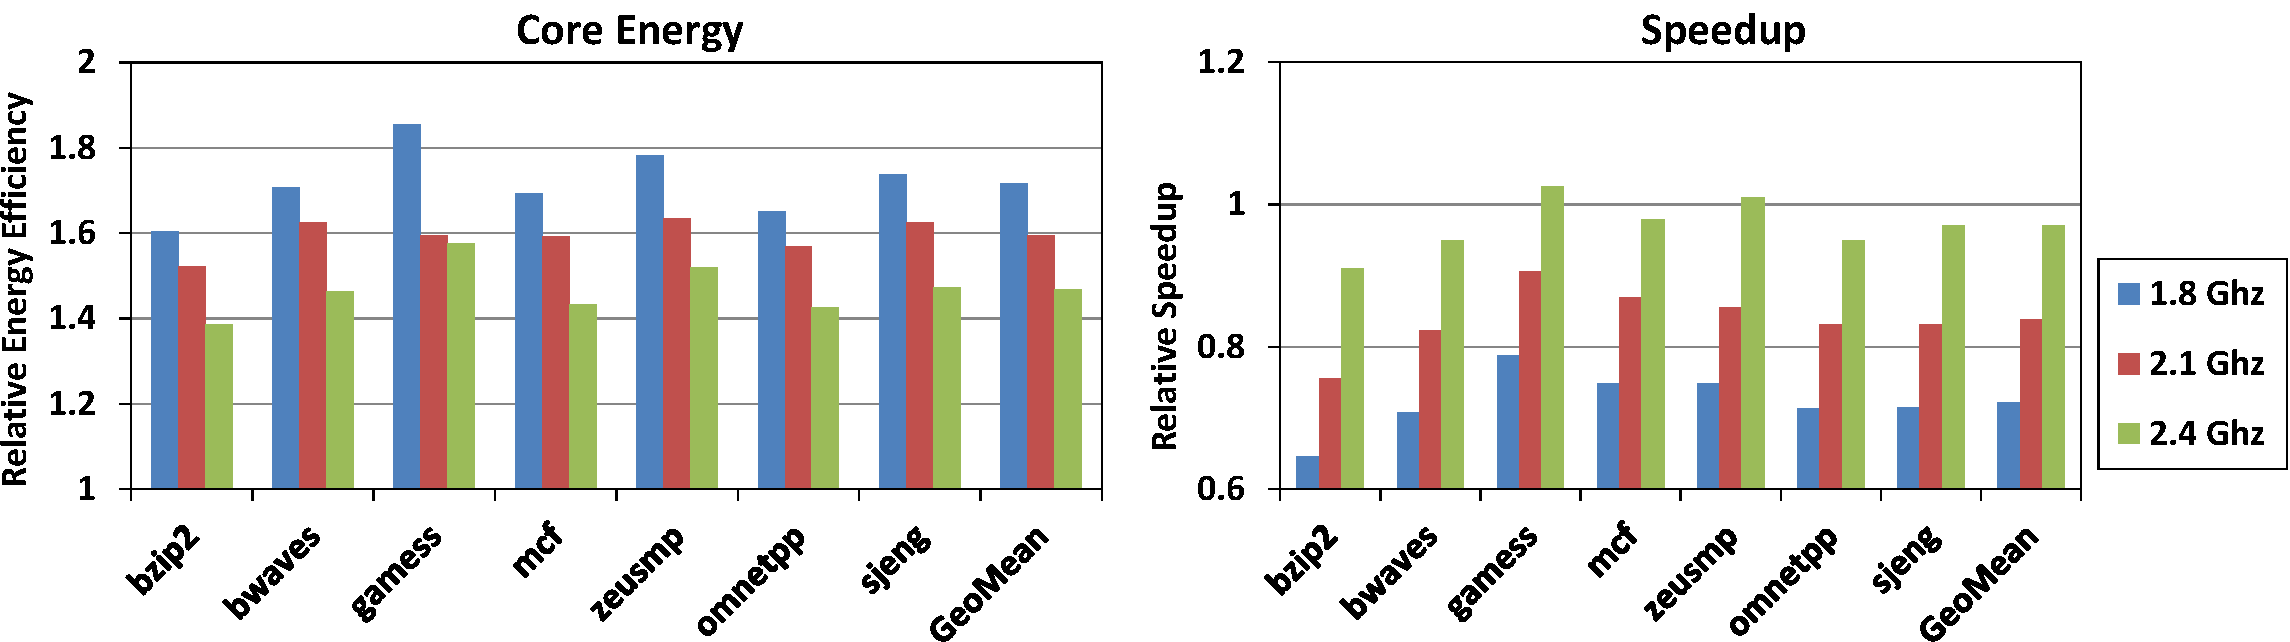
\includegraphics[width=\linewidth]{figs/user-spec-crop.pdf}
  \end{center}
	\vspace{-0.1in}
  \caption{SPEC2006 run with user-space governor with frequency setting 1.8Ghz to 2.4Ghz}
  \label{fig:user-spec}
\end{figure*}

\begin{figure*}[h]
  \begin{center}
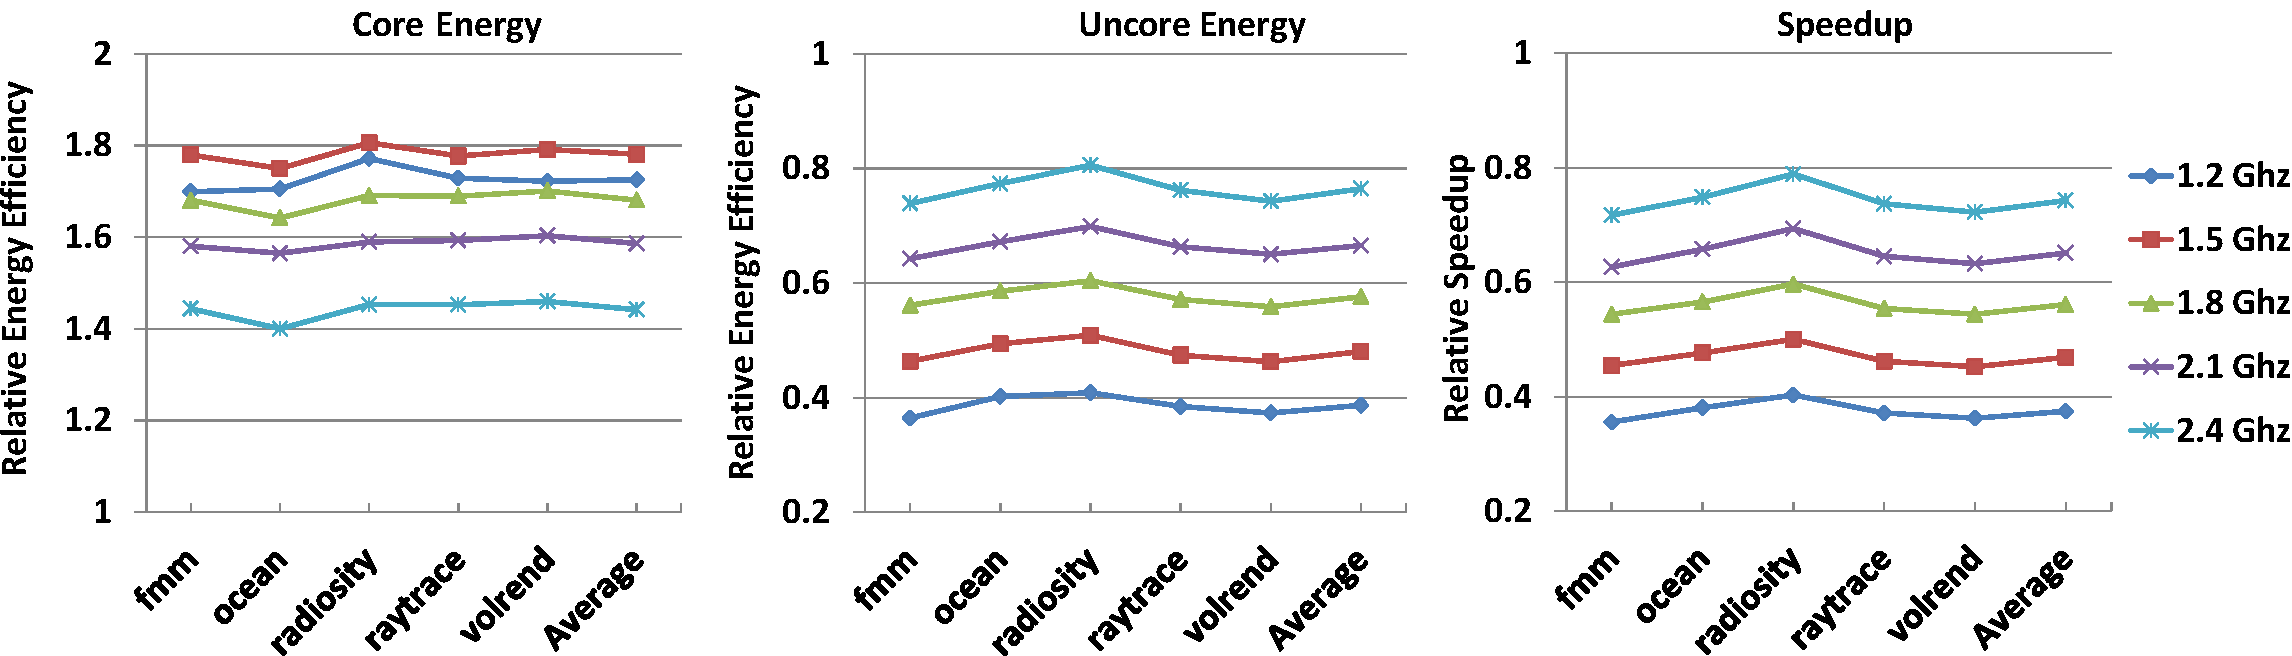
\includegraphics[width=\linewidth]{figs/user-splash-crop.pdf}
	\end{center}
	\vspace{-0.1in}
  \caption{SPLASH2 run with user-space governor with frequency setting 1.8Ghz to 2.1Ghz}
  \label{fig:user-splash}
\end{figure*}

\begin{figure*}[h]
  \begin{center}
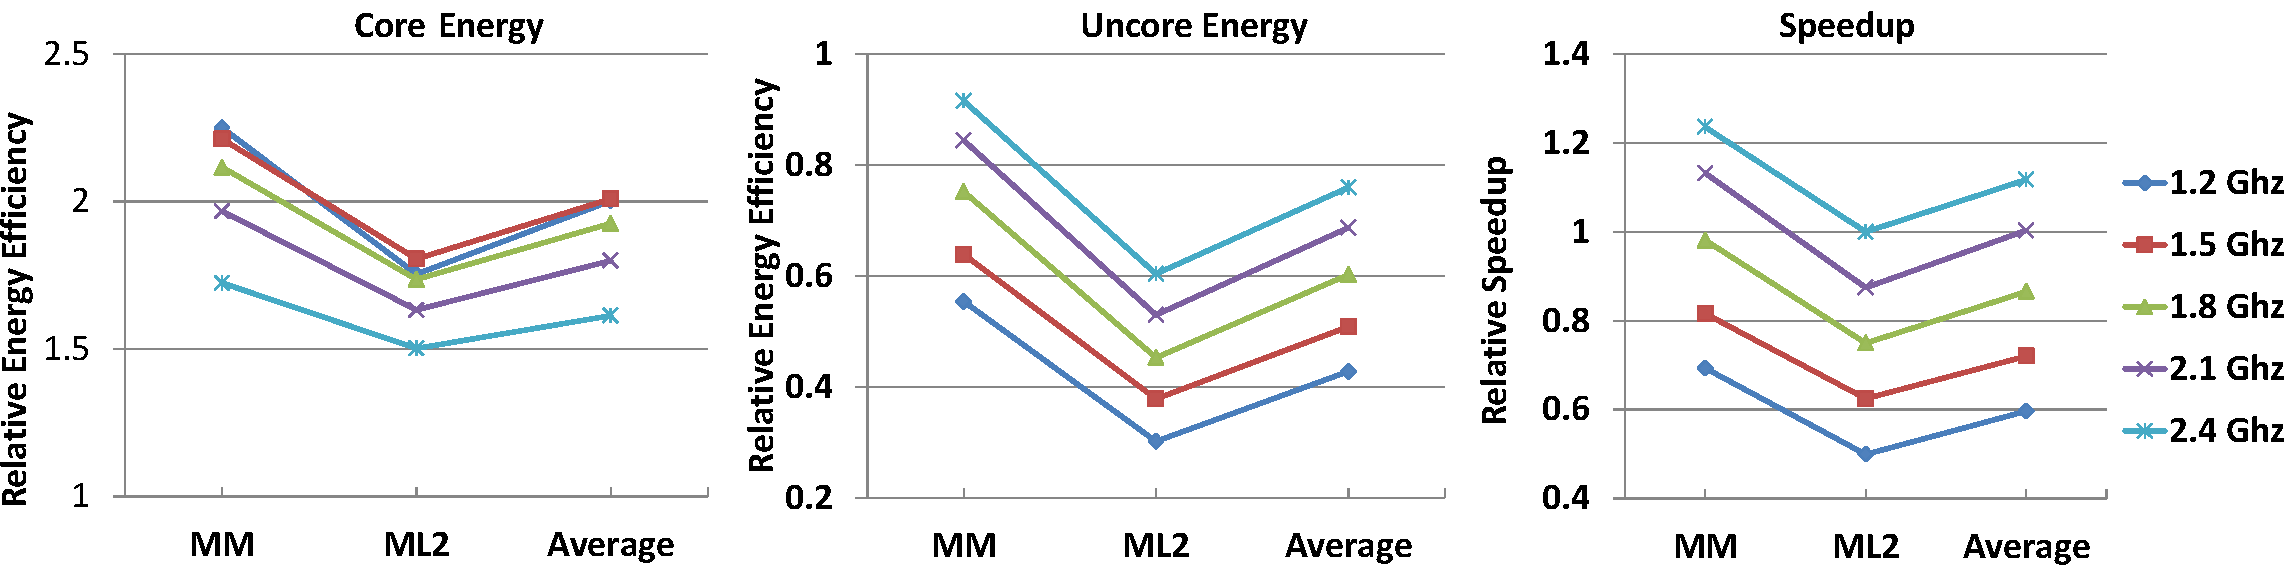
\includegraphics[width=\linewidth]{figs/user-micro-crop.pdf}
	\end{center}
	\vspace{-0.1in}
  \caption{MICRO-BENCH run with user-space governor with frequency setting 1.2Ghz to 1.8Ghz}
  \label{fig:user-micro}
\end{figure*}


In this section, we present our E-MOS model evaluation and the
results of the model i.e chosen frequency settings, for all the initial applications we profiled.
One important thing to remember is, we have optimized the model to 
work on energy as the first class objective and so the frequency setting chooses
by E-MOS is more aligned towards energy efficiency with reasonable performance loss.
We present our results based on each application type and the chosen frequency setting. 
We try to reason out why E-MOS would have chosen that setting and show the energy efficiency gains
for each category. For all the graphs, both the energy efficiency and performance are normalized
and are relative to the ondemand governor findings.

\subsection{Compute intensive workloads}
Figure~\ref{fig:user-spec} shows the relative energy efficiency and speedup
for SPEC2006 benchmarks which are mainly compute intensive workloads. 
E-MOS chose a frequency setting of 1.8Ghz to 2.4Ghz for best energy efficiency
among the available scalable frequency set. The geometric mean for 2.4Ghz indicates  
upto 1.4x of energy efficiency with just 3\% performance loss. Provided 
E-MOS was optimized for energy savings, 3\% performance loss with such significant energy gains
is a good indication. You can still boost the application till turbo boost capability
but you will lose lot of energy gains and so did E-MOS not choose setting
above 2.4Ghz as the power factor effects more to energy than the lower execution time.
With lower frequency of 1.8Ghz, you gain upto 1.6Ghz energy efficiency with performance loss
of 15\%. You might want to go to lower frequency settings when energy is atmost important with situations like
low battery in mobile phones.

\subsection{Cache sensitive workloads}
Figure~\ref{fig:user-splash} shows the relative energy efficiency and speedup
for SPLASH2 benchmarks which have both compute and cache sensitive workloads. 
E-MOS chose a frequency setting of 1.8Ghz to 2.1Ghz for best energy efficiency
among the available scalable frequency set. This rationale makes sense
as you want to slightly reduce the core frequency when most of the instructions
are accessing cache and especially with the random workload we saw in our case study,
you want to spend too many CPU cycles at higher frequency wasting energy.
The geometric mean for 2.1Ghz indicates  
upto 1.5x of energy efficiency with just 4\% performance loss.
With one setting lower, for 1.8Ghz you can gain energy efficiency upto 1.62x and a 9\% performance loss.
We believe for cache workloads 2.1Ghz is good, as modern processors are equipped with
prefect hing and out of order execution mechanisms which hides the cache latency effectively and thus 
want to be executing at slightly higher frequency than 1.8Ghz.
This result was interestinng as we expected E-MOS to still choose a lower setting, but we 
got around 1.5x energy efficiency with a higher setting.

\subsection{Memory intensive workloads}
Figure~\ref{fig:user-micro} shows the relative energy efficiency and speedup
for SPEC2006 benchmarks which are mainly compute intensive workloads. 
E-MOS chose a frequency setting of 1.8Ghz to 2.4Ghz for best energy efficiency
among the available scalable frequency set. The geometric mean for 2.4Ghz indicates  
upto 1.4x of energy efficiency with just 3\% performance loss. Provided 
E-MOS was optimized for energy savings, 3\% performance loss with such significant energy gains
is a good indication. You can still boost the application till turbo boost capability
but you will lose lot of energy gains and so did E-MOS not choose setting
above 2.4Ghz as the power factor effects more to energy than the lower execution time.
With lower frequency of 1.8Ghz, you gain upto 1.6Ghz energy efficiency with performance loss
of 15\%. You might want to go to lower frequency settings when energy is atmost important with situations like
low battery in mobile phones.

